\chapter{Results}

%	<Paragraph> Overview of results
This chapter provides results of the $k$-{\sc Sat} execution test from the previous chapter.  We consider the results of the test and provide analysis of the algorithm metrics.  

	\section{Algorithm metric comparison}
	
%		<Paragraph> Summary of measured metrics
This section provides results from the simulation.  We provide the analysis for the molecular operations.  These include counts of append, extract, mix, purify, splice, and split.  Presentation of actual computation time and required memory for the solution representation allow for comparison of algorithms.

\FloatBarrier
		
%\subsection{Append}

%%%%%%%%%%%%%%%%%%%%%%%%%%%%%%%%%
\begin{figure}[htdp]

\reversemarginpar{
\textbf{Append} is an operation that concatenates molecules. \\

The Distribution algorithm is exponential in the number of appends.  The operation count for append depends on the parsing order of the \textsf{CNF} expression.\\

Lipton's and Ogihara-Ray's algorithms use a fixed amount of appends.  This depends on the number of variables and clauses present in the \textsf{CNF} expression.
}

\begin{center}

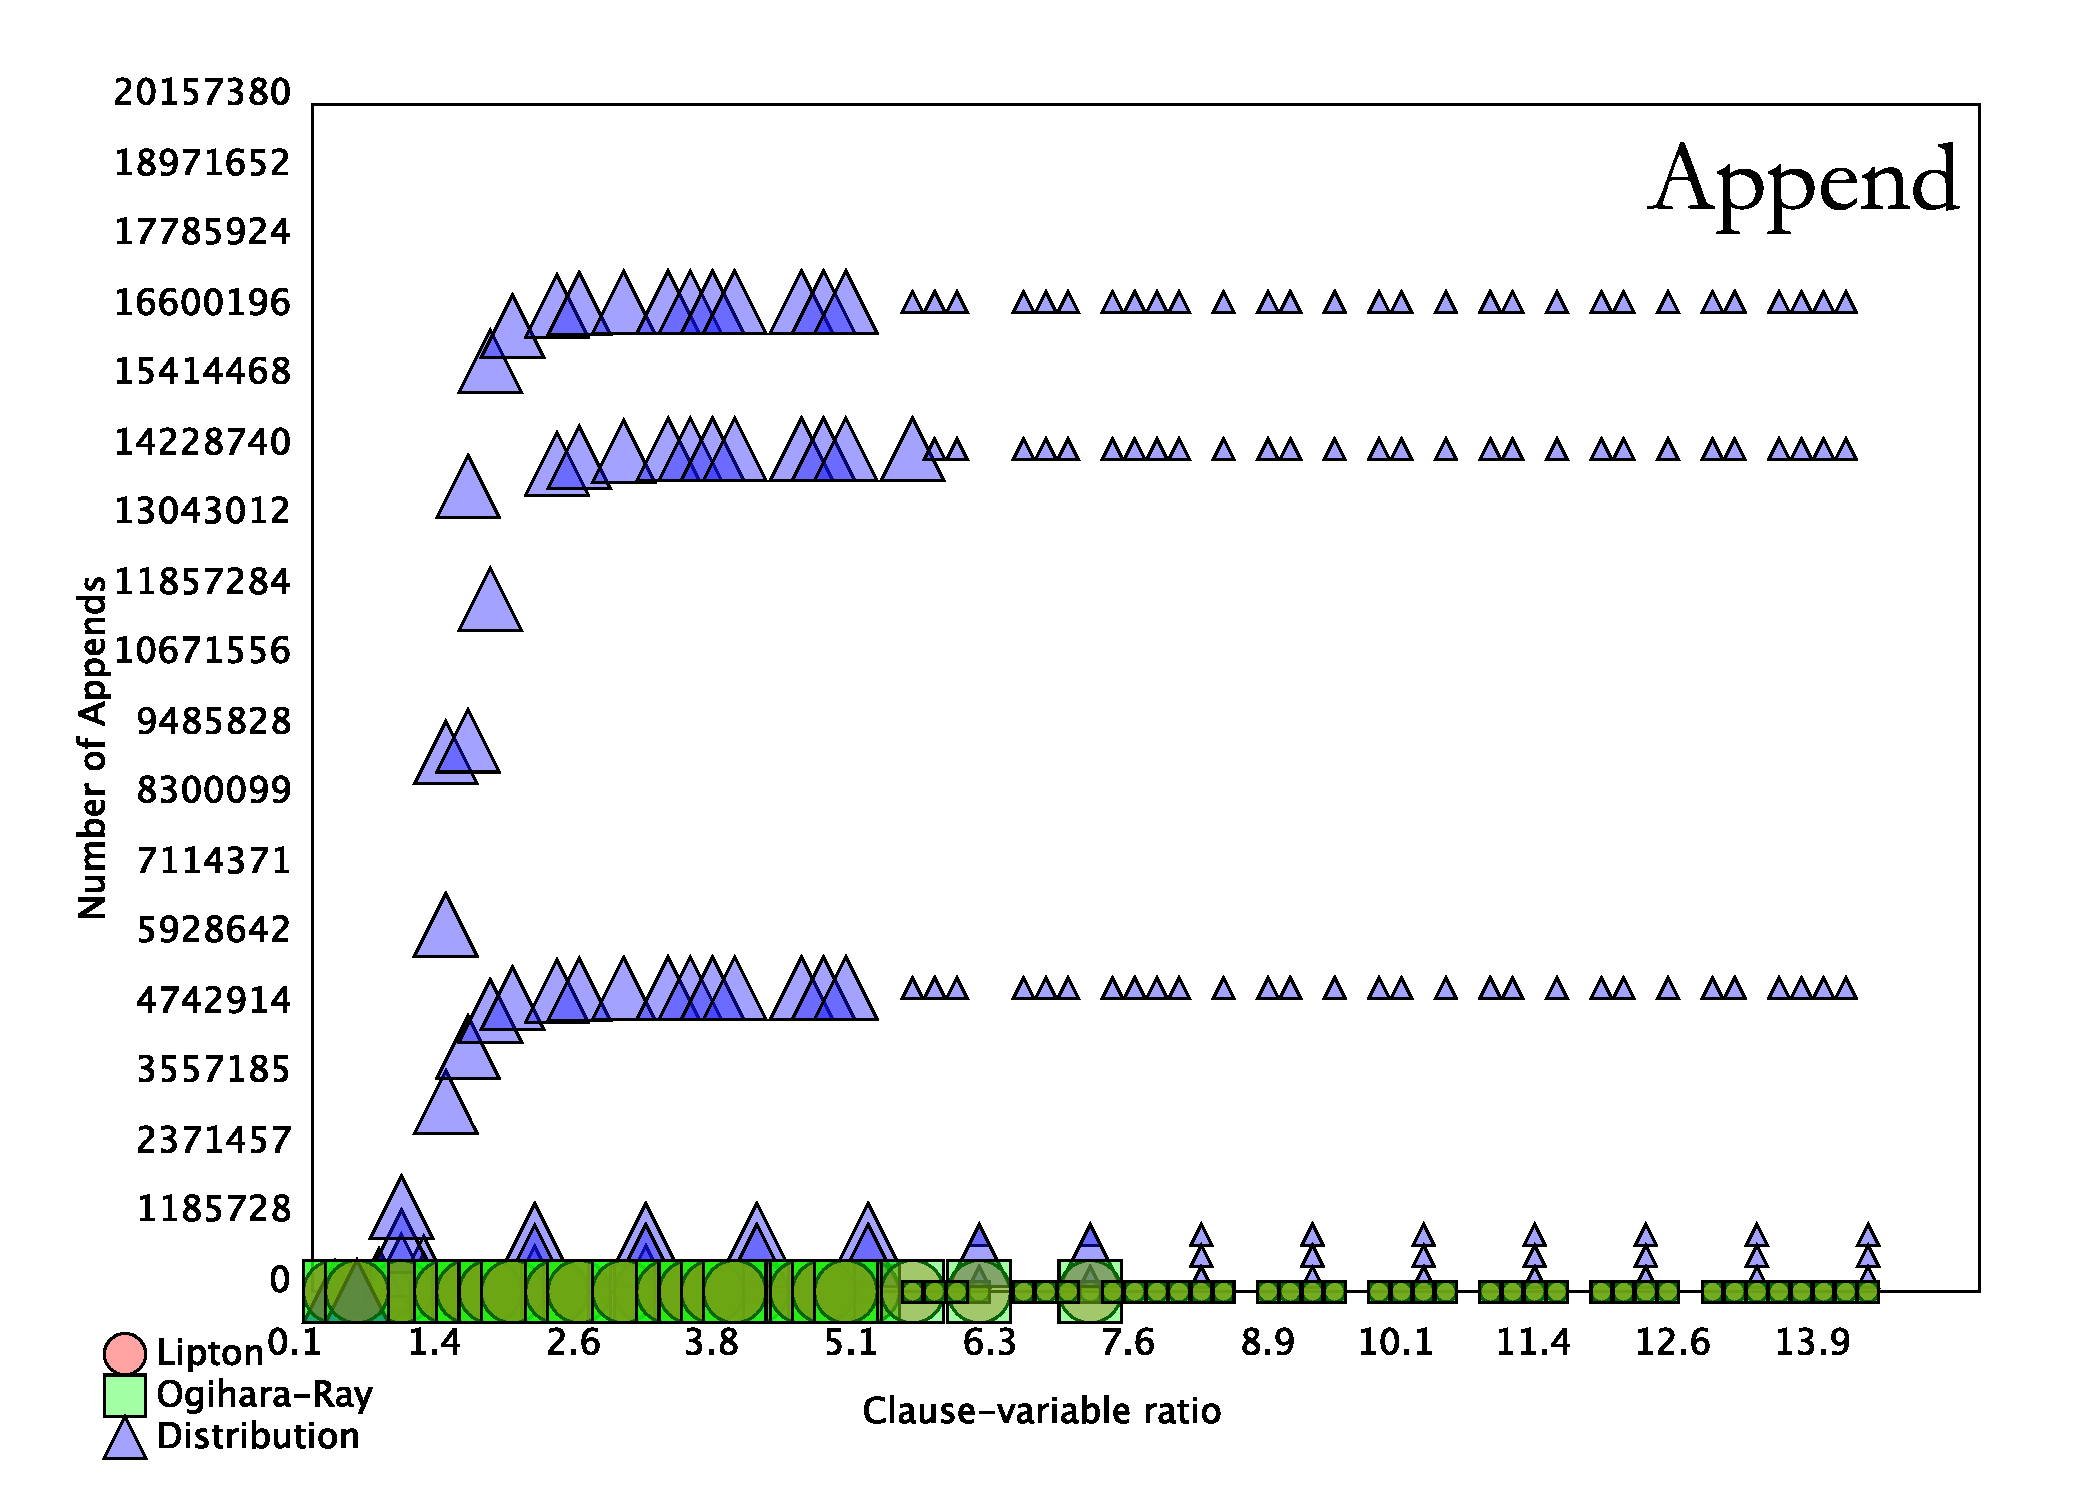
\includegraphics[width=1.1\textwidth]{./figures/metricOutput/Append.pdf}

\caption{Clause to variable ratio $\alpha$ vs. Number of appends }
\label{appendFig}
\end{center}
\end{figure}
%%%%%%%%%%%%%%%%%%%%%%%%%%%%%%%%%

\FloatBarrier
			
%\subsection{Extract}
%%%%%%%%%%%%%%%%%%%%%%%%%%%%%%%%%
\begin{figure}[htdp]

\reversemarginpar{

\textbf{Extract} is an operation that filters strings.\\

Ogihara-Ray's algorithm requires the greatest amount of extracts.  Lipton's algorithm is linear on $\alpha$ and varies a constant amount from Ogihara-Ray's algorithm.\\

The Distribution algorithm does not require extract.

}

\begin{center}

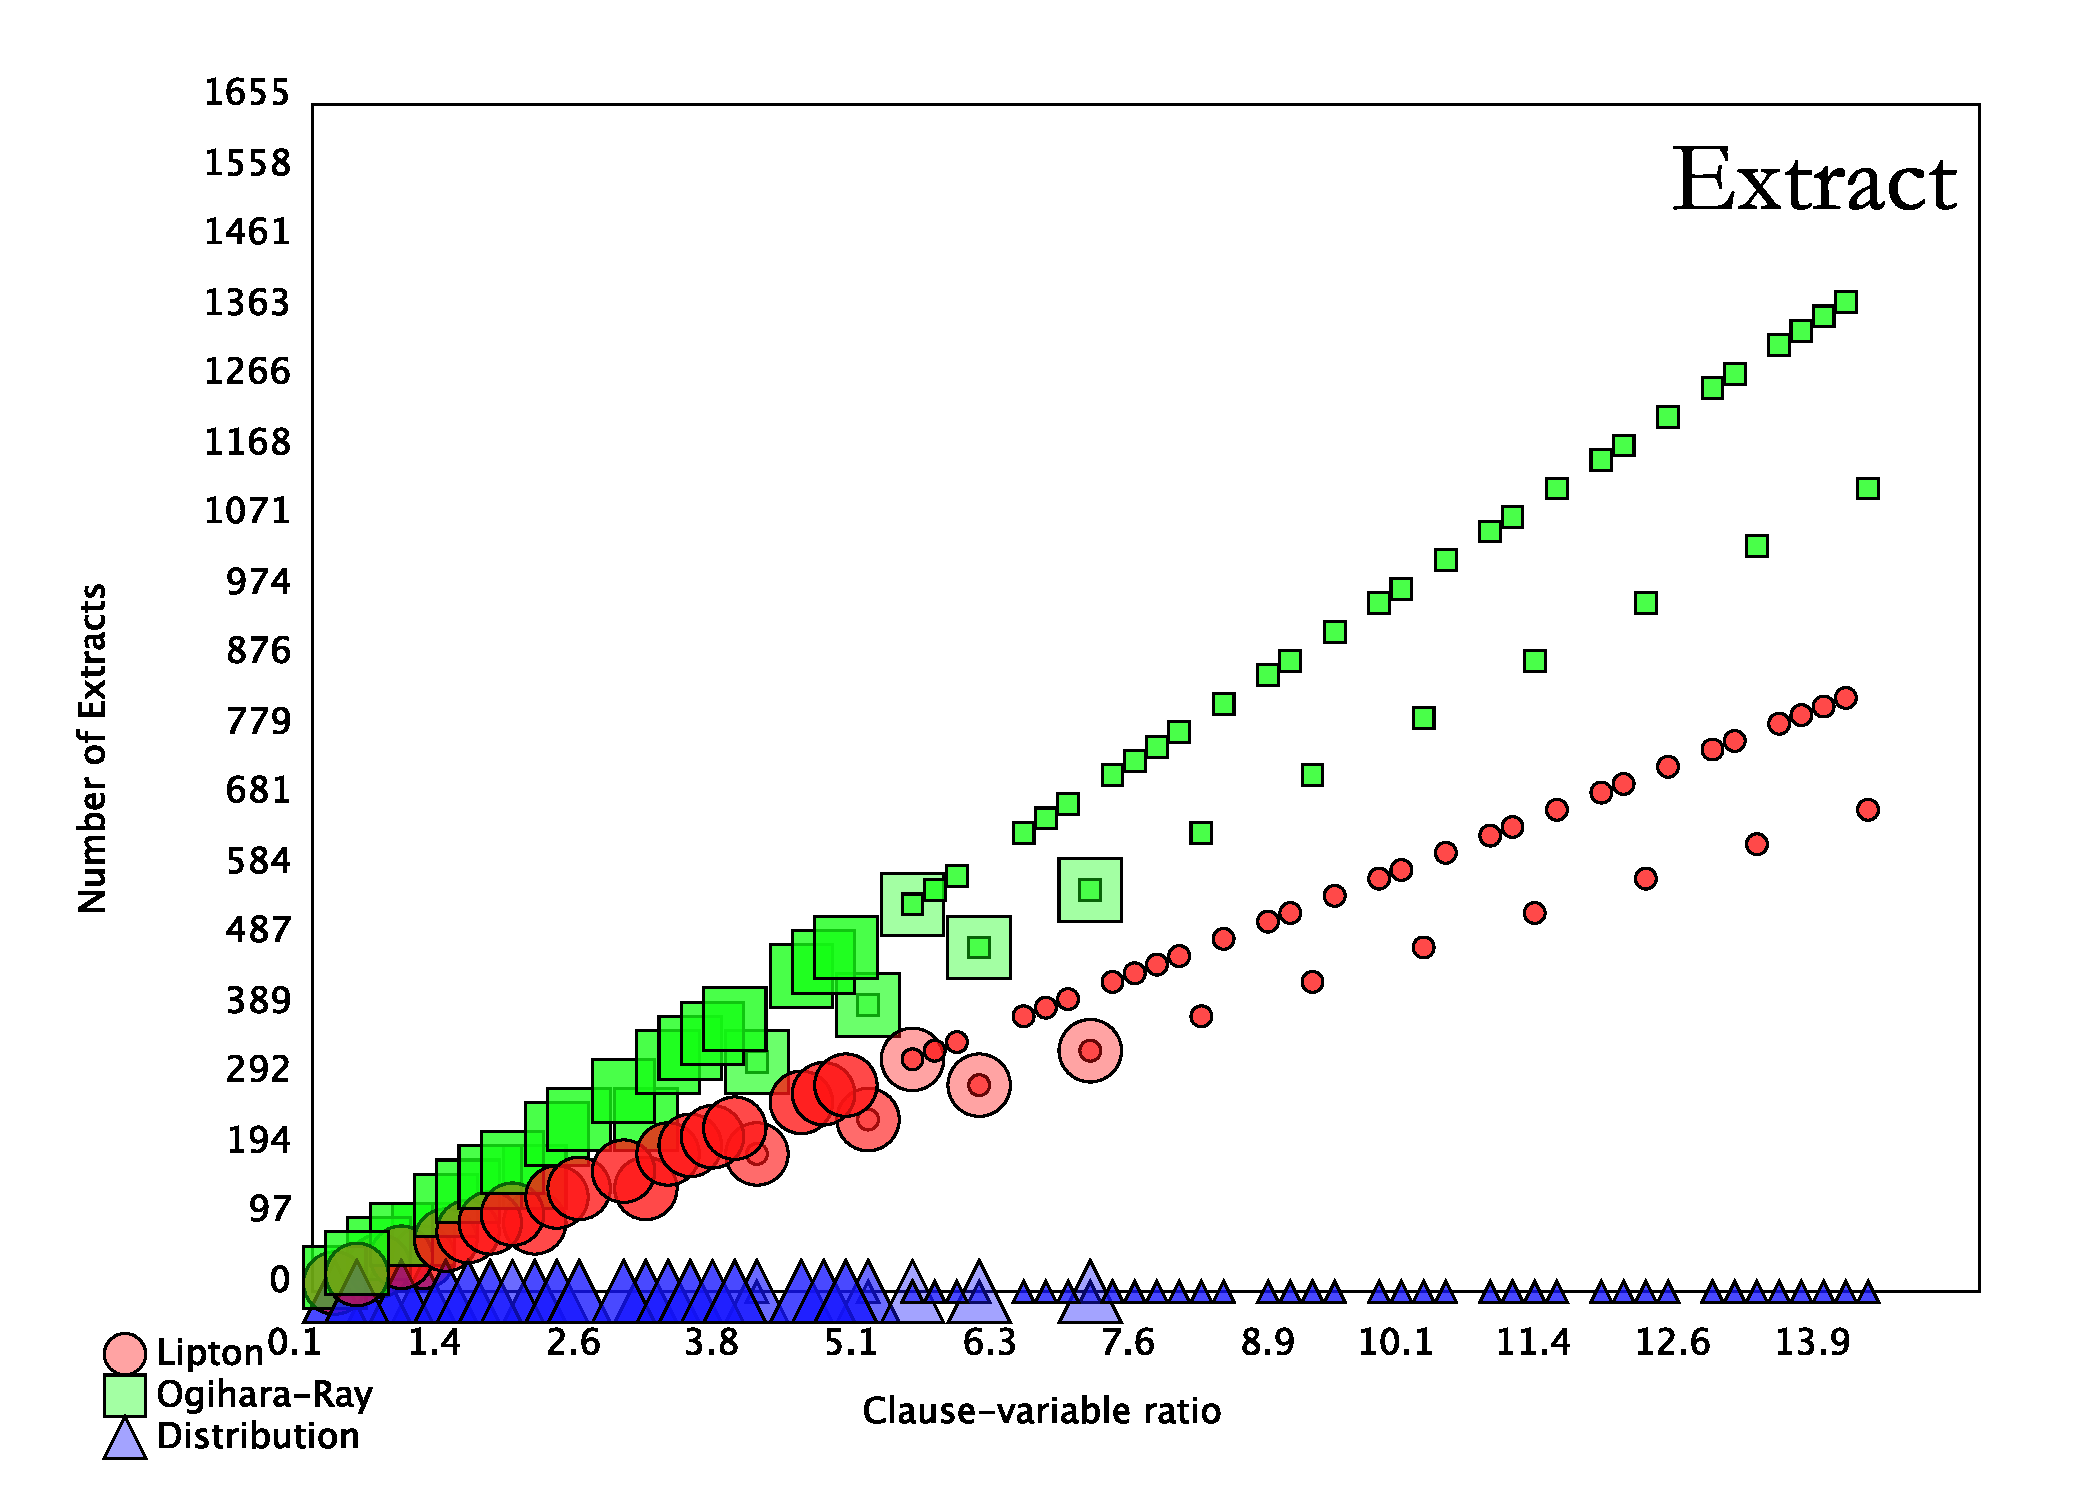
\includegraphics[width=1.1\textwidth]{./figures/metricOutput/Extract.pdf}

\caption{Clause to variable ratio $\alpha$ vs. Number of extracts }
\label{extractFig}
\end{center}
\end{figure}
%%%%%%%%%%%%%%%%%%%%%%%%%%%%%%%%%
\FloatBarrier			
			
%\subsection{Mix}
%%%%%%%%%%%%%%%%%%%%%%%%%%%%%%%%%
\begin{figure}[htdp]

\reversemarginpar{
\textbf{Mix} is an operation that combines two tubes.\\

Lipton's algorithm requires a linear amount of mixes on $\alpha$.  The Distribution algorithm also requires a linear number of mixes, varying by a constant factor from Lipton's algorithm.\\

Ogihara-Ray's algorithm requires a constant amount of mixes on $\alpha$.
}

\begin{center}

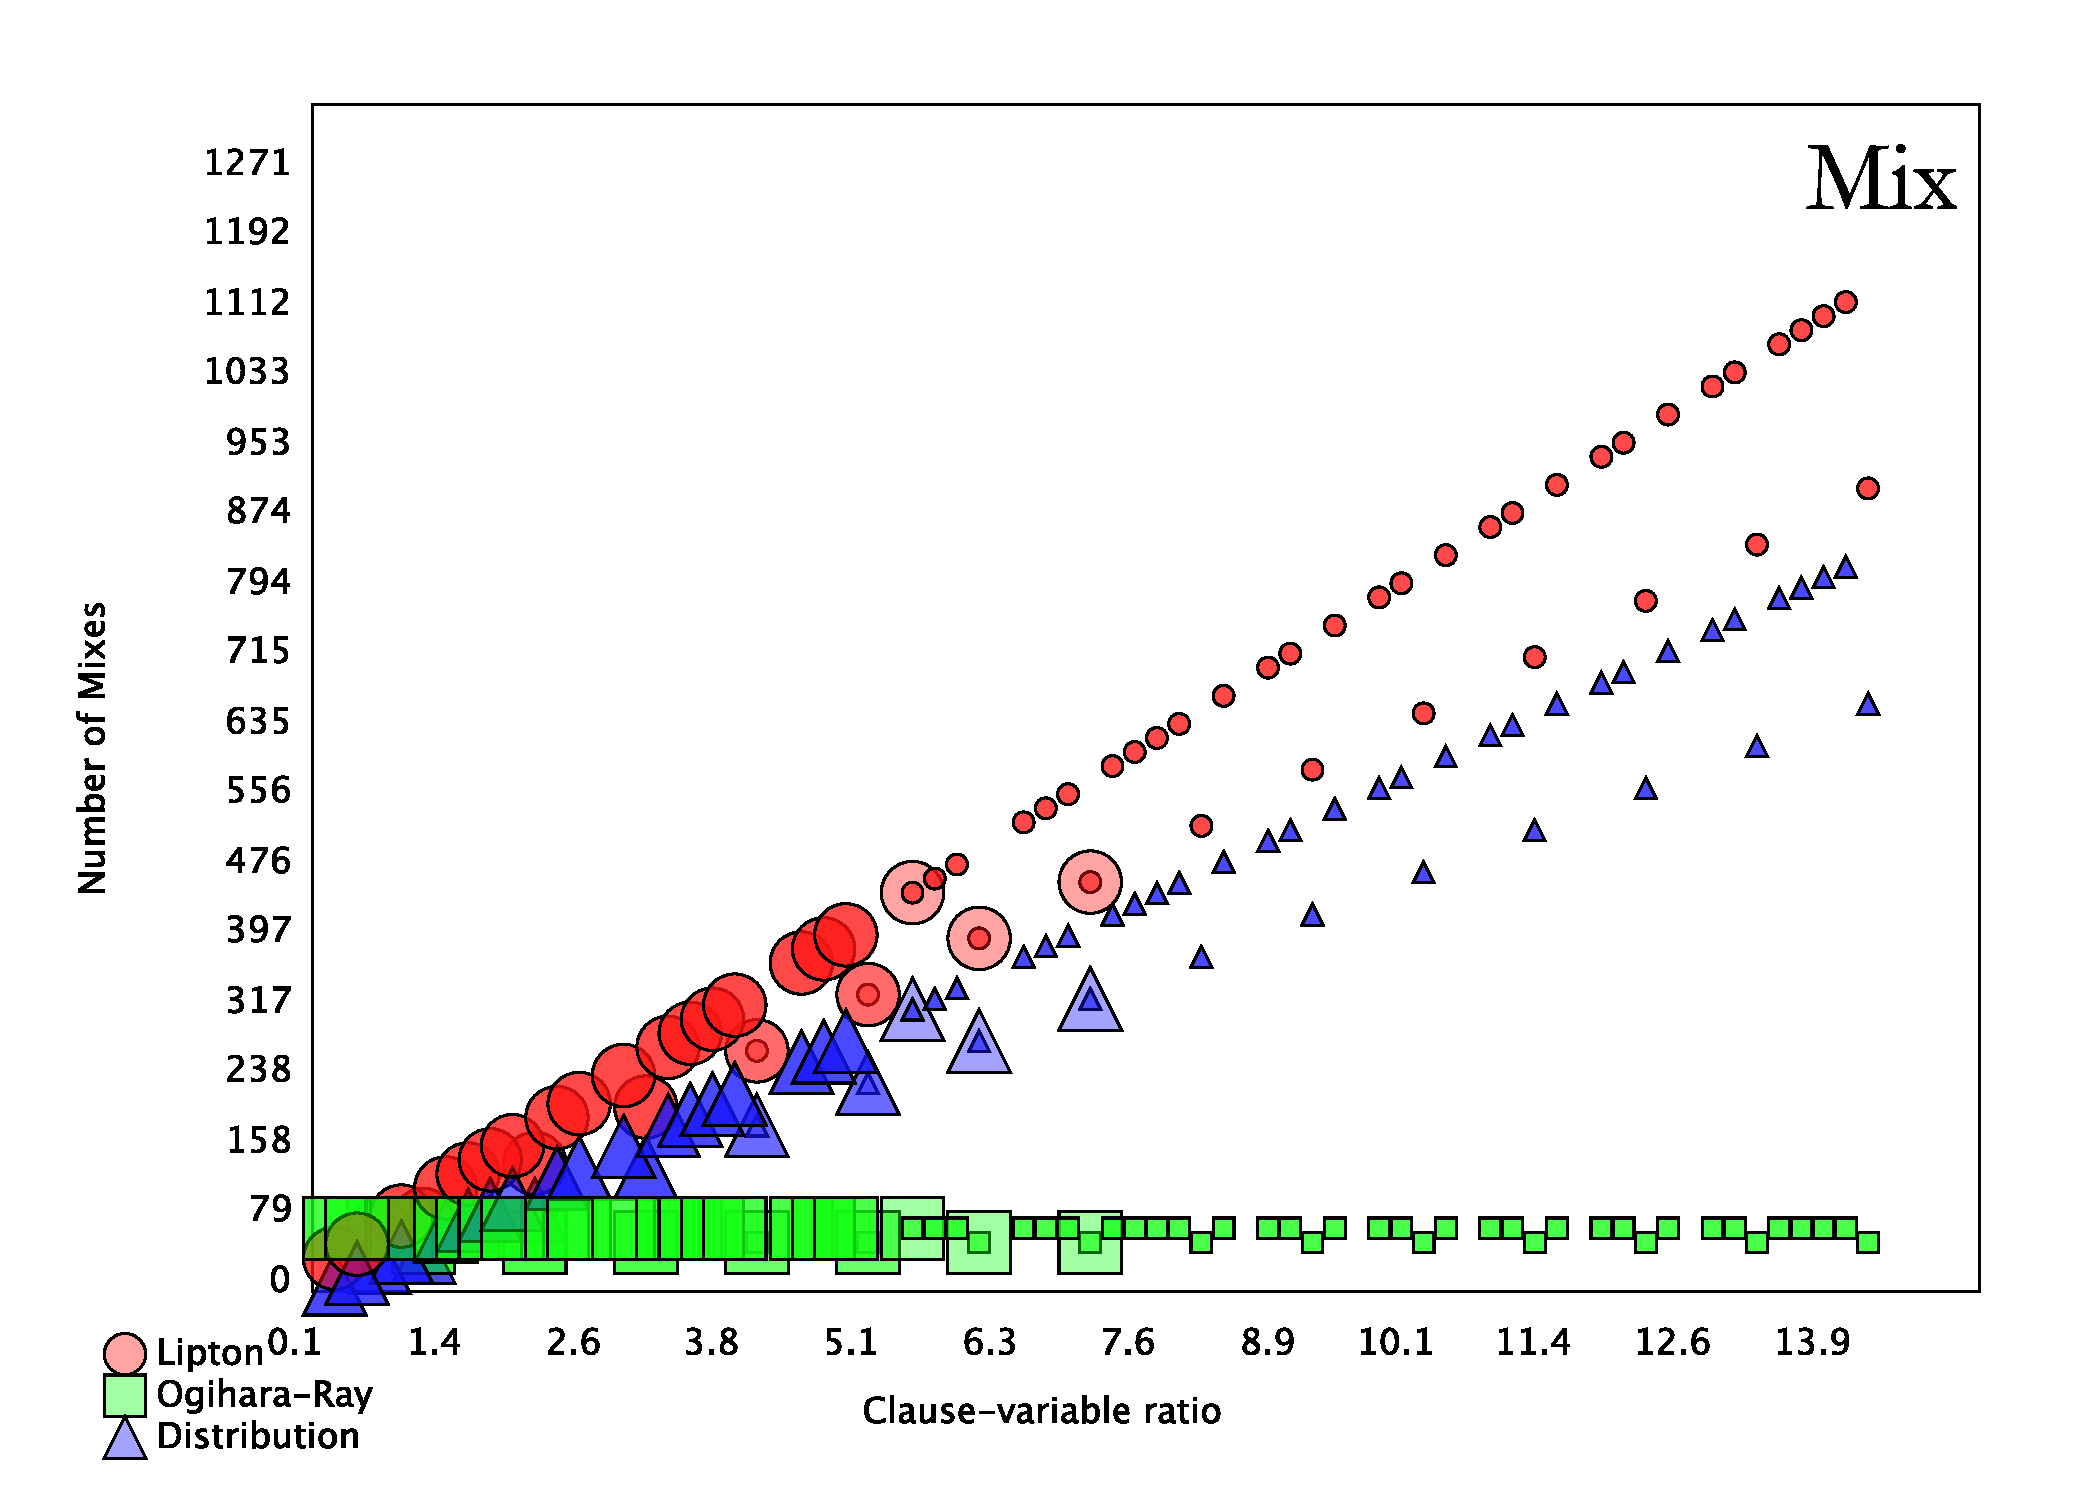
\includegraphics[width=1.1\textwidth]{./figures/metricOutput/Mix.pdf}

\caption{Clause to variable ratio $\alpha$ vs. Number of mixes }
\label{mixFig}
\end{center}
\end{figure}
%%%%%%%%%%%%%%%%%%%%%%%%%%%%%%%%%
\FloatBarrier

%\subsection{Purify}
%%%%%%%%%%%%%%%%%%%%%%%%%%%%%%%%%
\begin{figure}[htdp]

\reversemarginpar{
\textbf{Purify} is an operation that ensures equal portions of each independent string.\\

All three algorithms operate with a  linear  number of purifications on $\alpha$.  Ogihara-Ray's algorithm requires the greatest amount of purifications.  The purifications vary by a constant amount when compared with Lipton's and the Distribution algorithms.

 }

\begin{center}

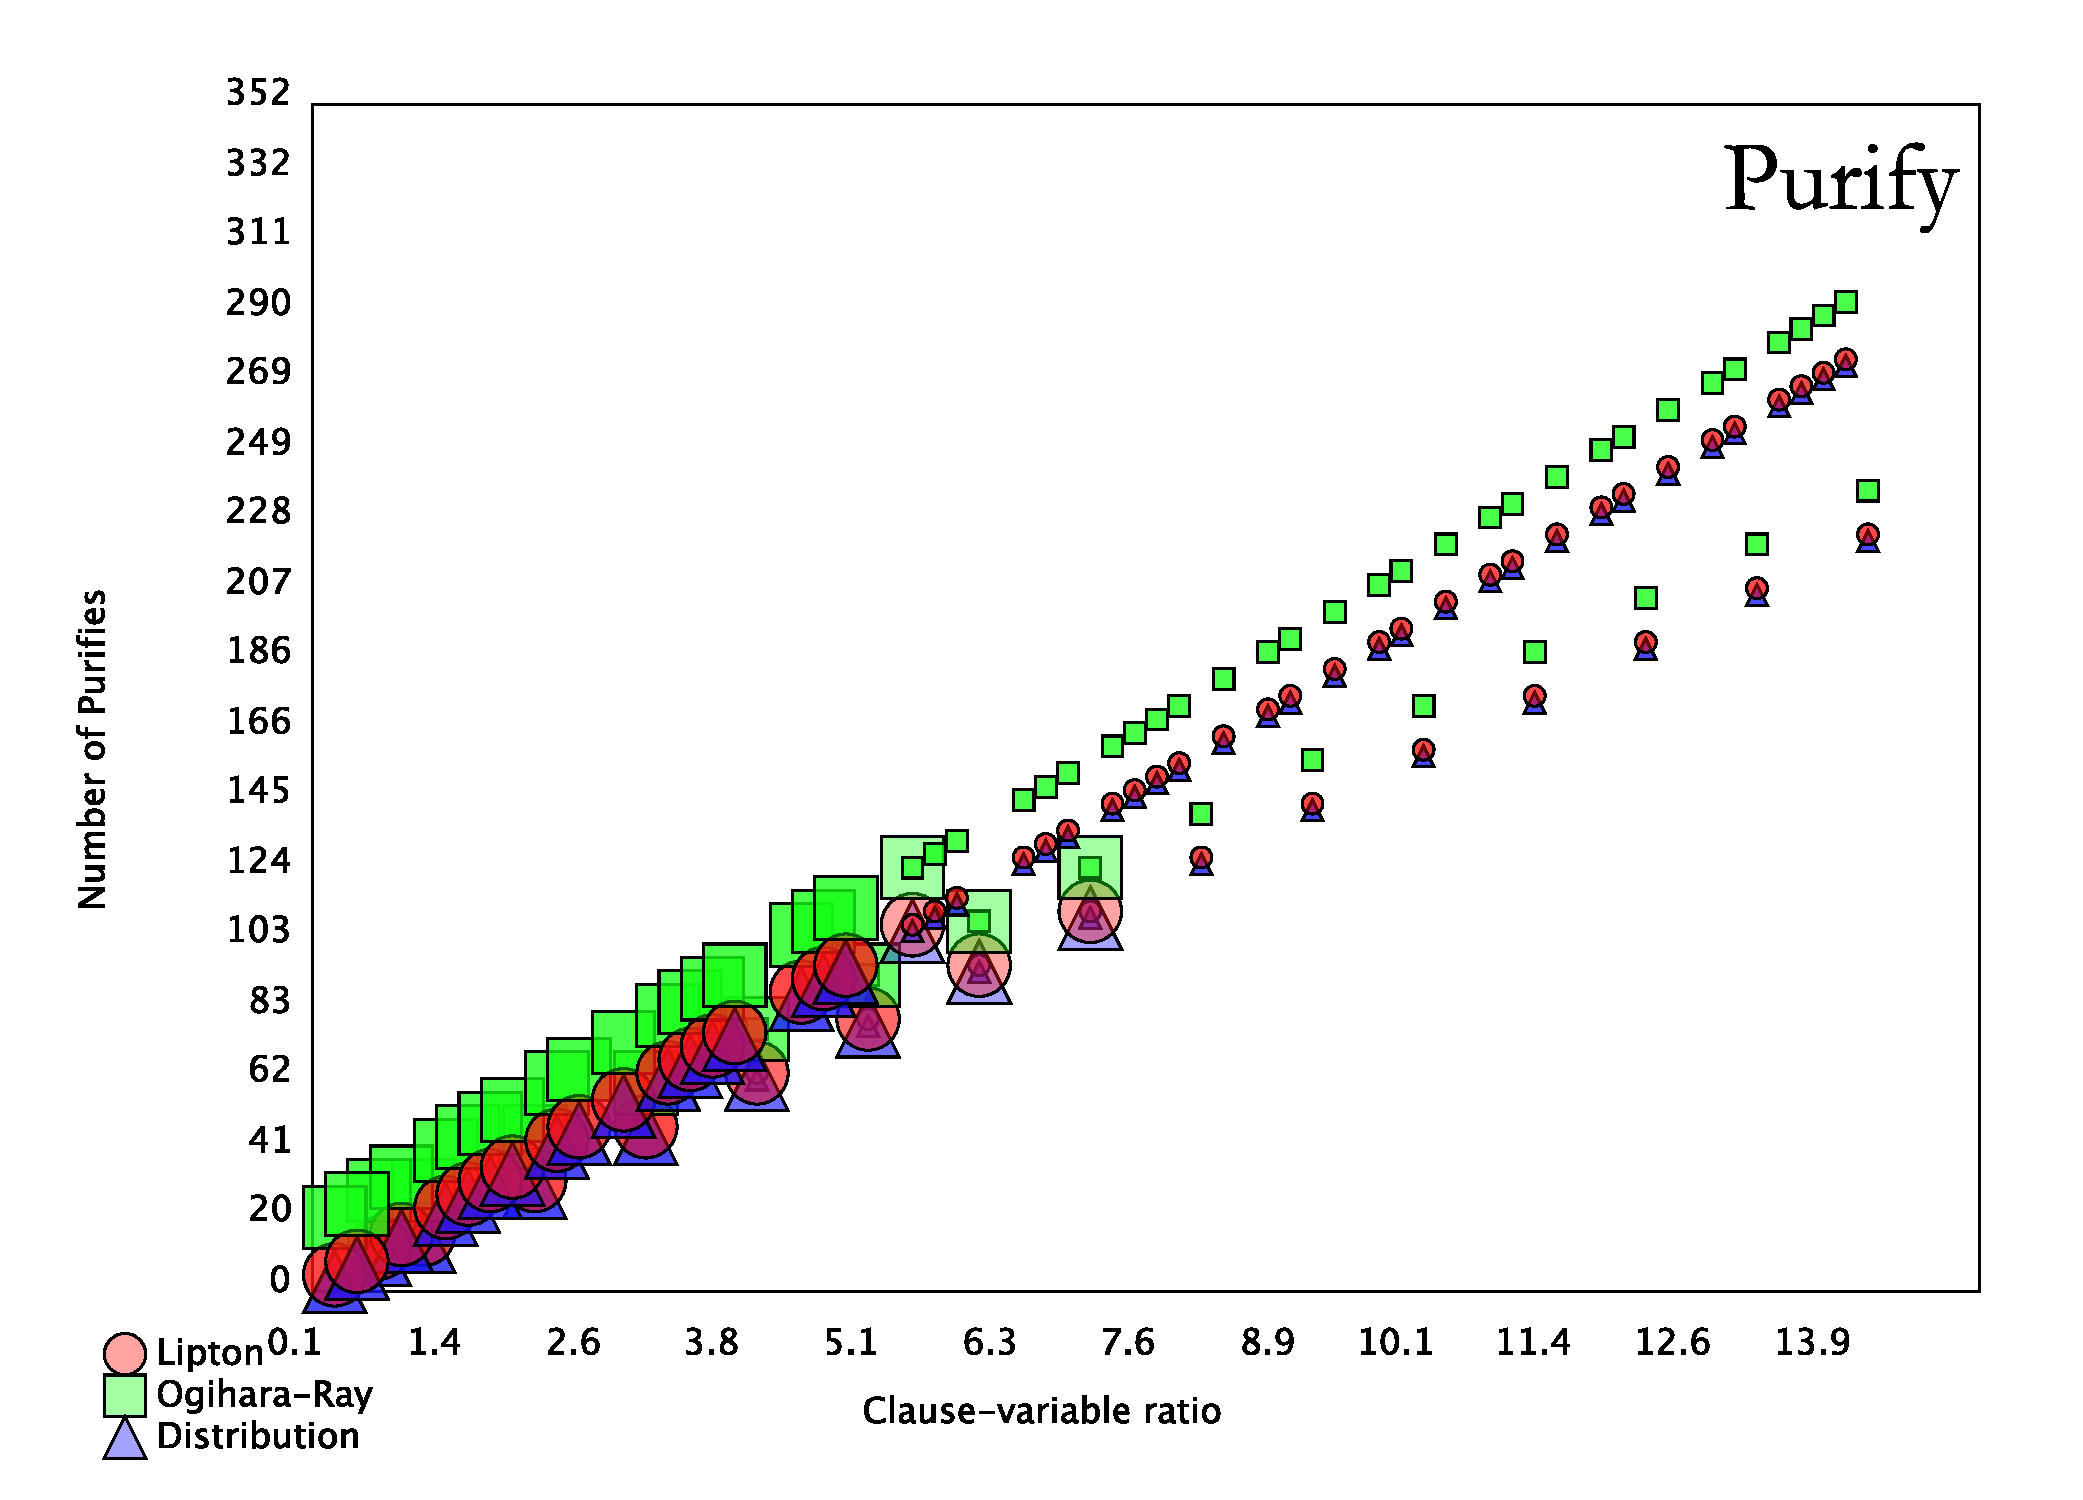
\includegraphics[width=1.1\textwidth]{./figures/metricOutput/Purify.pdf}

\caption{Clause to variable ratio $\alpha$ vs. Number of purifies }
\label{purifyFig}
\end{center}
\end{figure}
%%%%%%%%%%%%%%%%%%%%%%%%%%%%%%%%%
\FloatBarrier

%\subsection{Splice}
%%%%%%%%%%%%%%%%%%%%%%%%%%%%%%%%%
\begin{figure}[htdp]

\reversemarginpar{
\textbf{Splice} is an operation that inserts a string at a targeted location.\\

The Distribution algorithm is exponential in the number of splices.  The number of splices depends on the parsing order of the \textsf{CNF} expression.  Each split requires reassembly, accomplished with two appends.  Figure \ref{appendFig} shows the number of appends.\\

Lipton's and Ogihara-Ray's algorithms do not require splice the splice operator.
}

\begin{center}

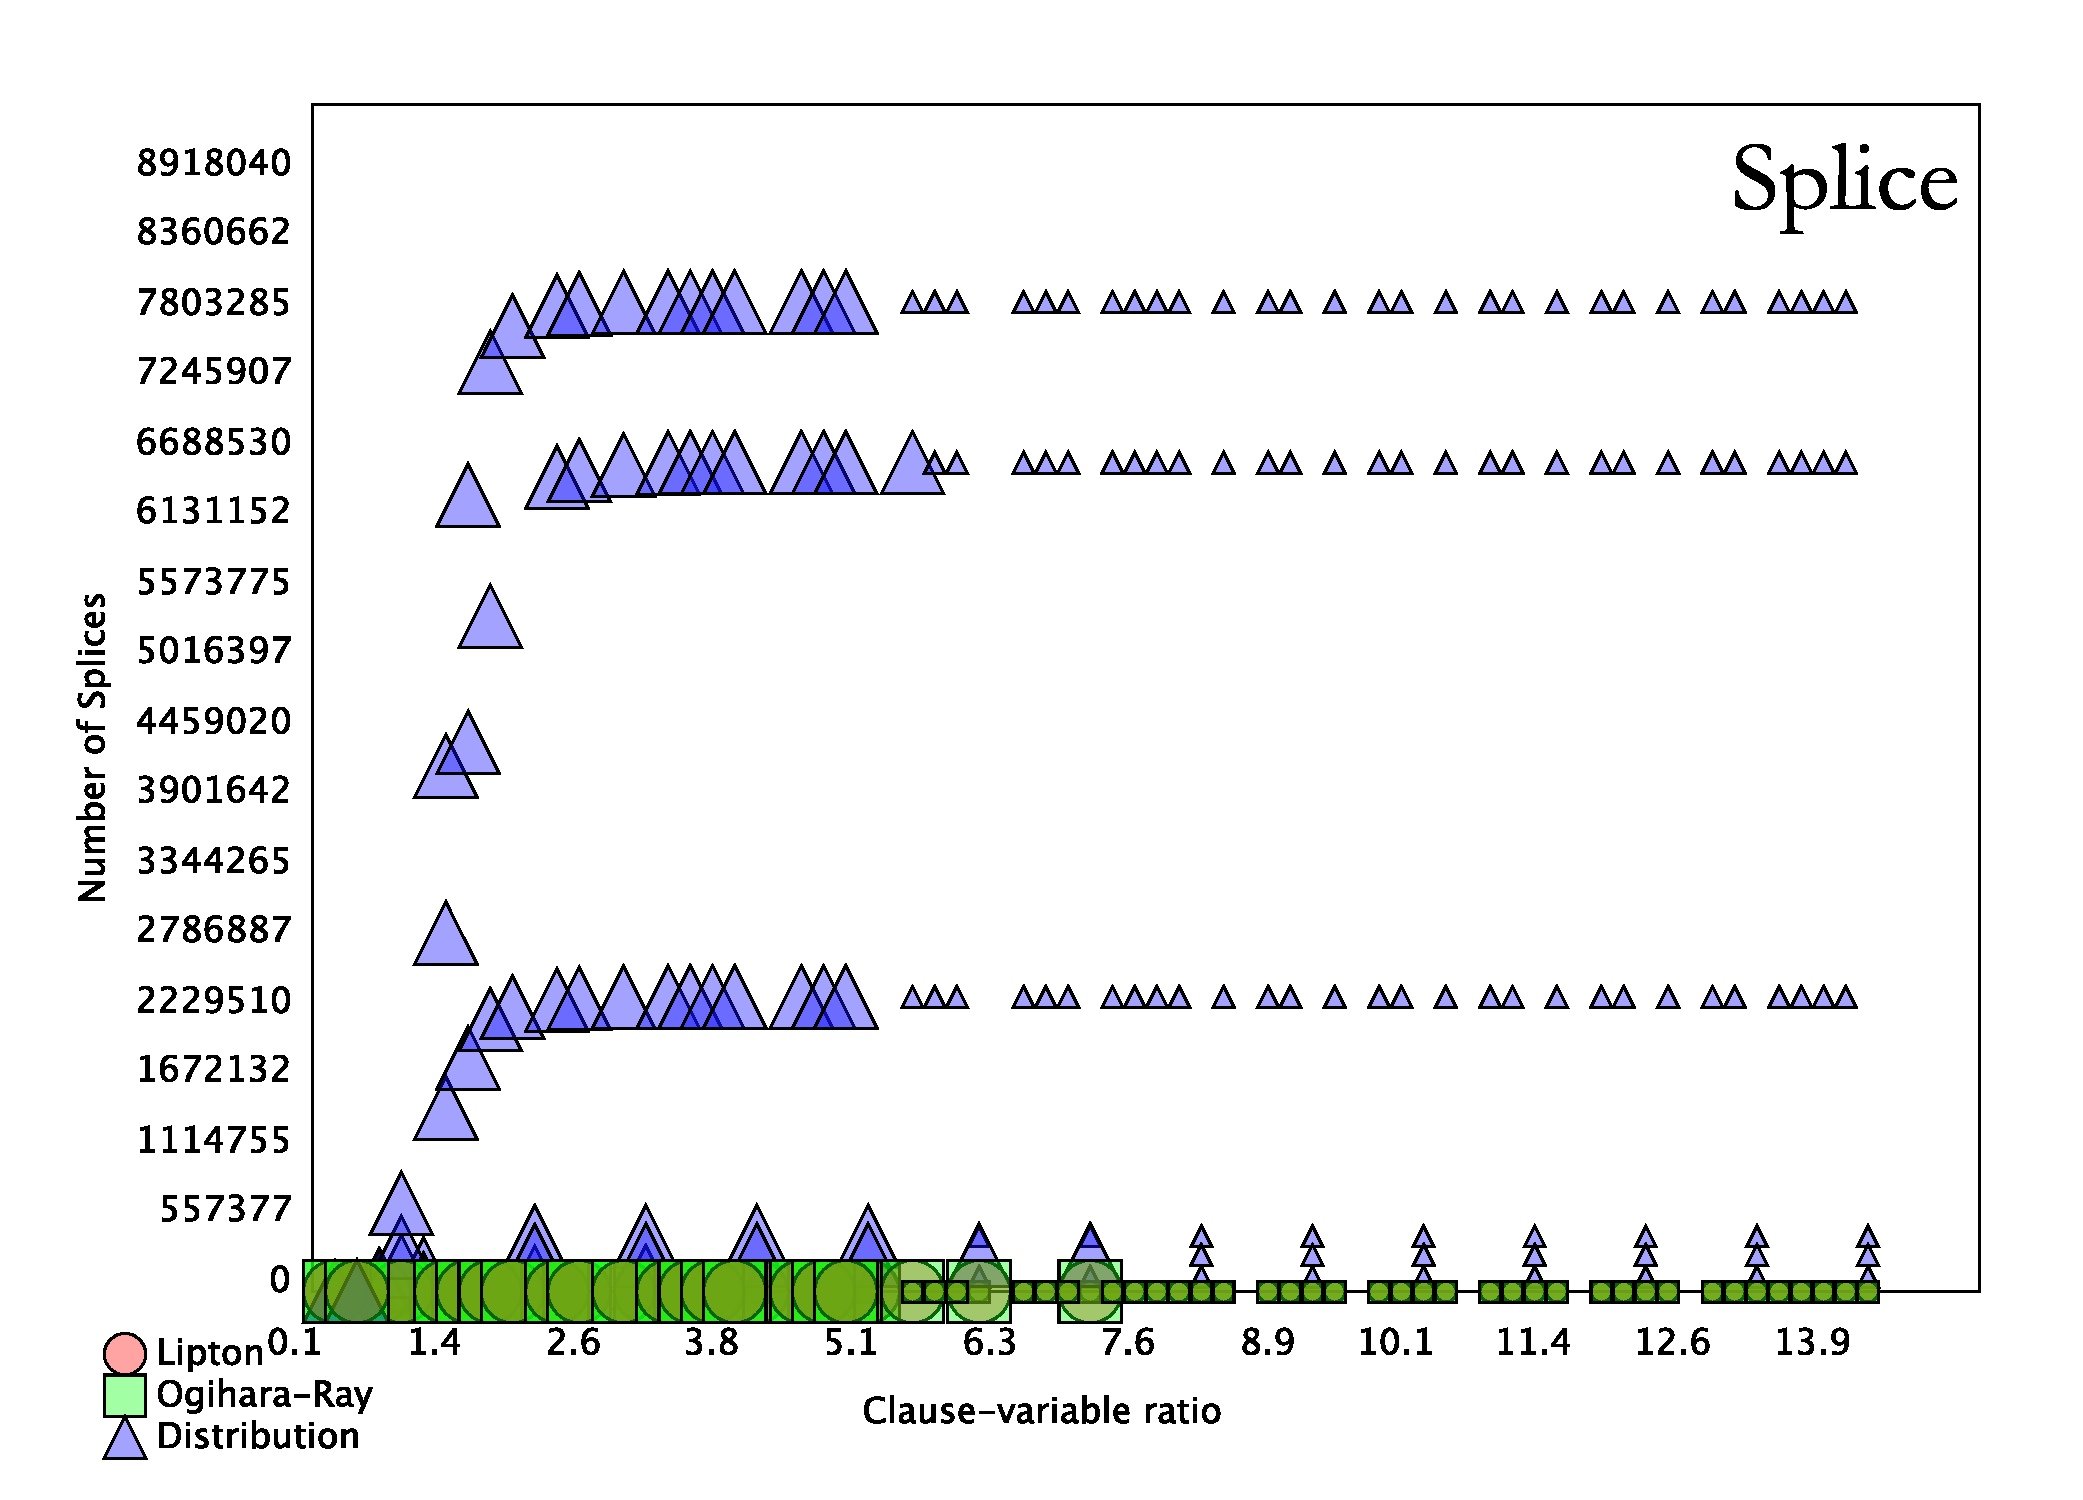
\includegraphics[width=1.1\textwidth]{./figures/metricOutput/Splice.pdf}

\caption{Clause to variable ratio $\alpha$ vs. Number of splices }
\label{spliceFig}
\end{center}
\end{figure}
%%%%%%%%%%%%%%%%%%%%%%%%%%%%%%%%%
\FloatBarrier

%\subsection{Split}
%%%%%%%%%%%%%%%%%%%%%%%%%%%%%%%%%
\begin{figure}[htdp]

\reversemarginpar{

\textbf{Split} is an operation that portions a tube into two exact copes.\\

Distribution requires a linear number of splits.\\

Lipton's and Ogihara-Ray's algorithms are constant in splits based the number of variables.
 }

\begin{center}

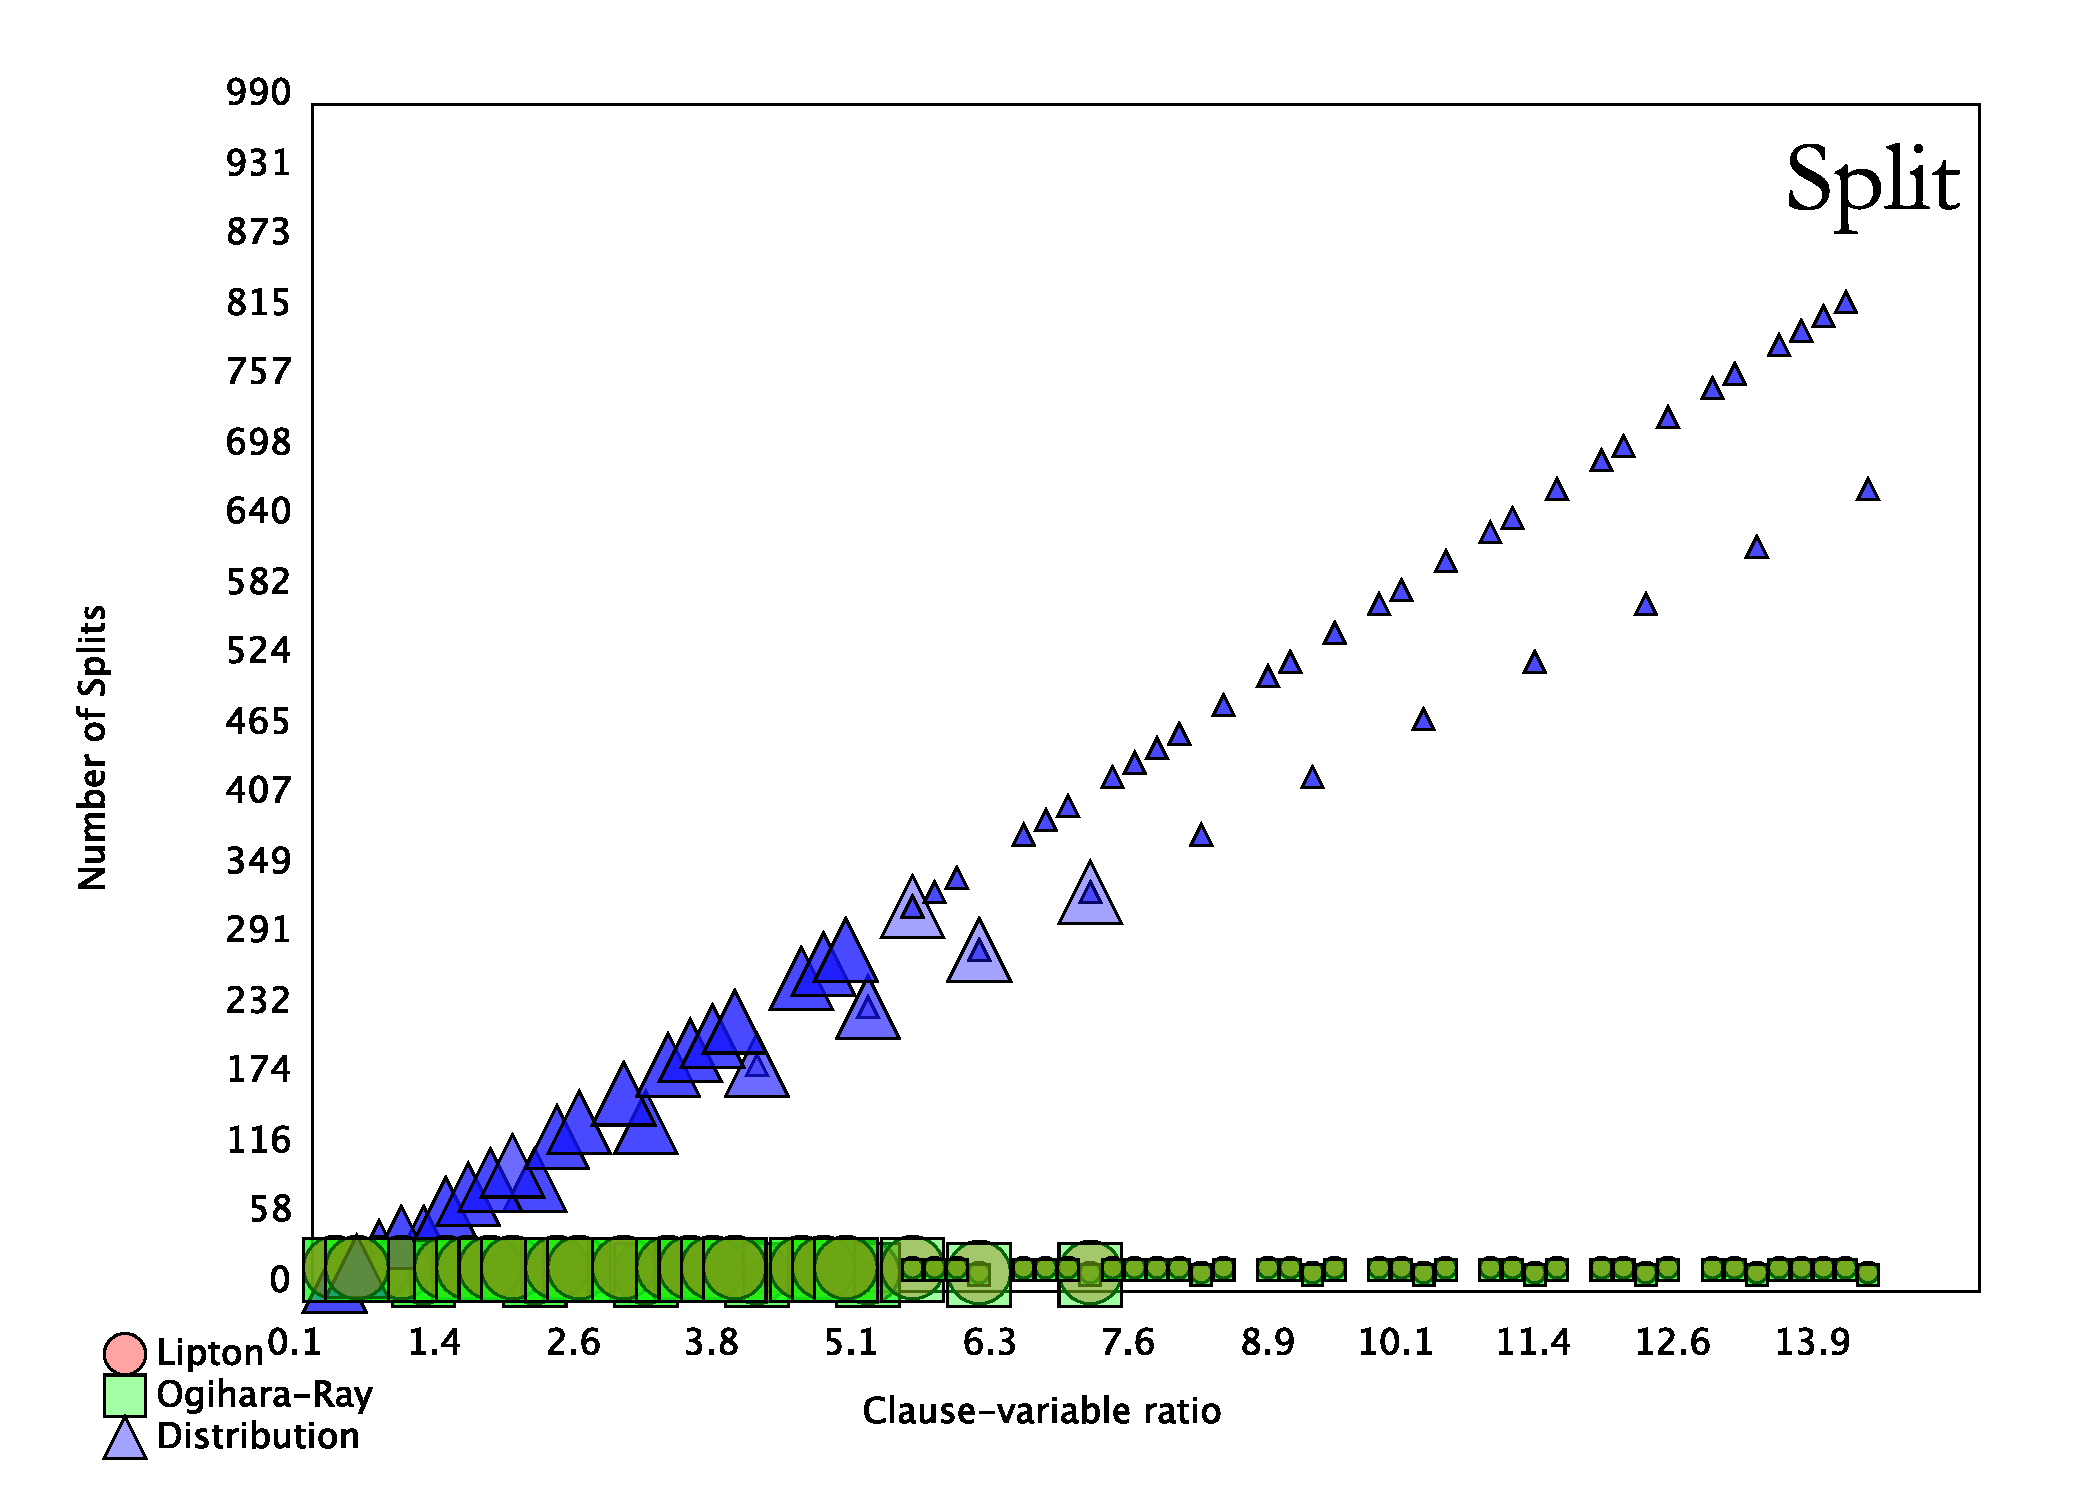
\includegraphics[width=1.1\textwidth]{./figures/metricOutput/Split.pdf}

\caption{Clause to variable ratio $\alpha$ vs. Number of splits }
\label{splitFig}
\end{center}
\end{figure}
%%%%%%%%%%%%%%%%%%%%%%%%%%%%%%%%%
\FloatBarrier

			
%\subsection{Time}
%%%%%%%%%%%%%%%%%%%%%%%%%%%%%%%%%
\begin{figure}[htdp]

\reversemarginpar{
\textbf{Time} is a measurement of algorithm execution in seconds.\\

Ogihara-Ray's algorithm requires the least amount of time.  In cases where the {\sc Satisfiability} instance is under-constrained, where more possible solutions occur, the algorithm takes the greatest amount of time.  Less pruning occurs in over-constrained instances, reducing the execution time of test instances.

Lipton's algorithm executes in exponential time with $\alpha \approx [4.2, 8.2]$ taking the longest.  This is within the phase-transition region for $3$-{\sc Sat}.\\

The Distribution algorithm executes in exponential time, and performs better than Lipton's algorithm for low conflict ratios.  However over the entire sweep performs worse than both Lipton's and Ogihara-Ray's algorithms.  It shares the same $\alpha \approx [4.2, 8.2]$ during the $3$-{\sc Sat} phase-transition.
}

\begin{center}

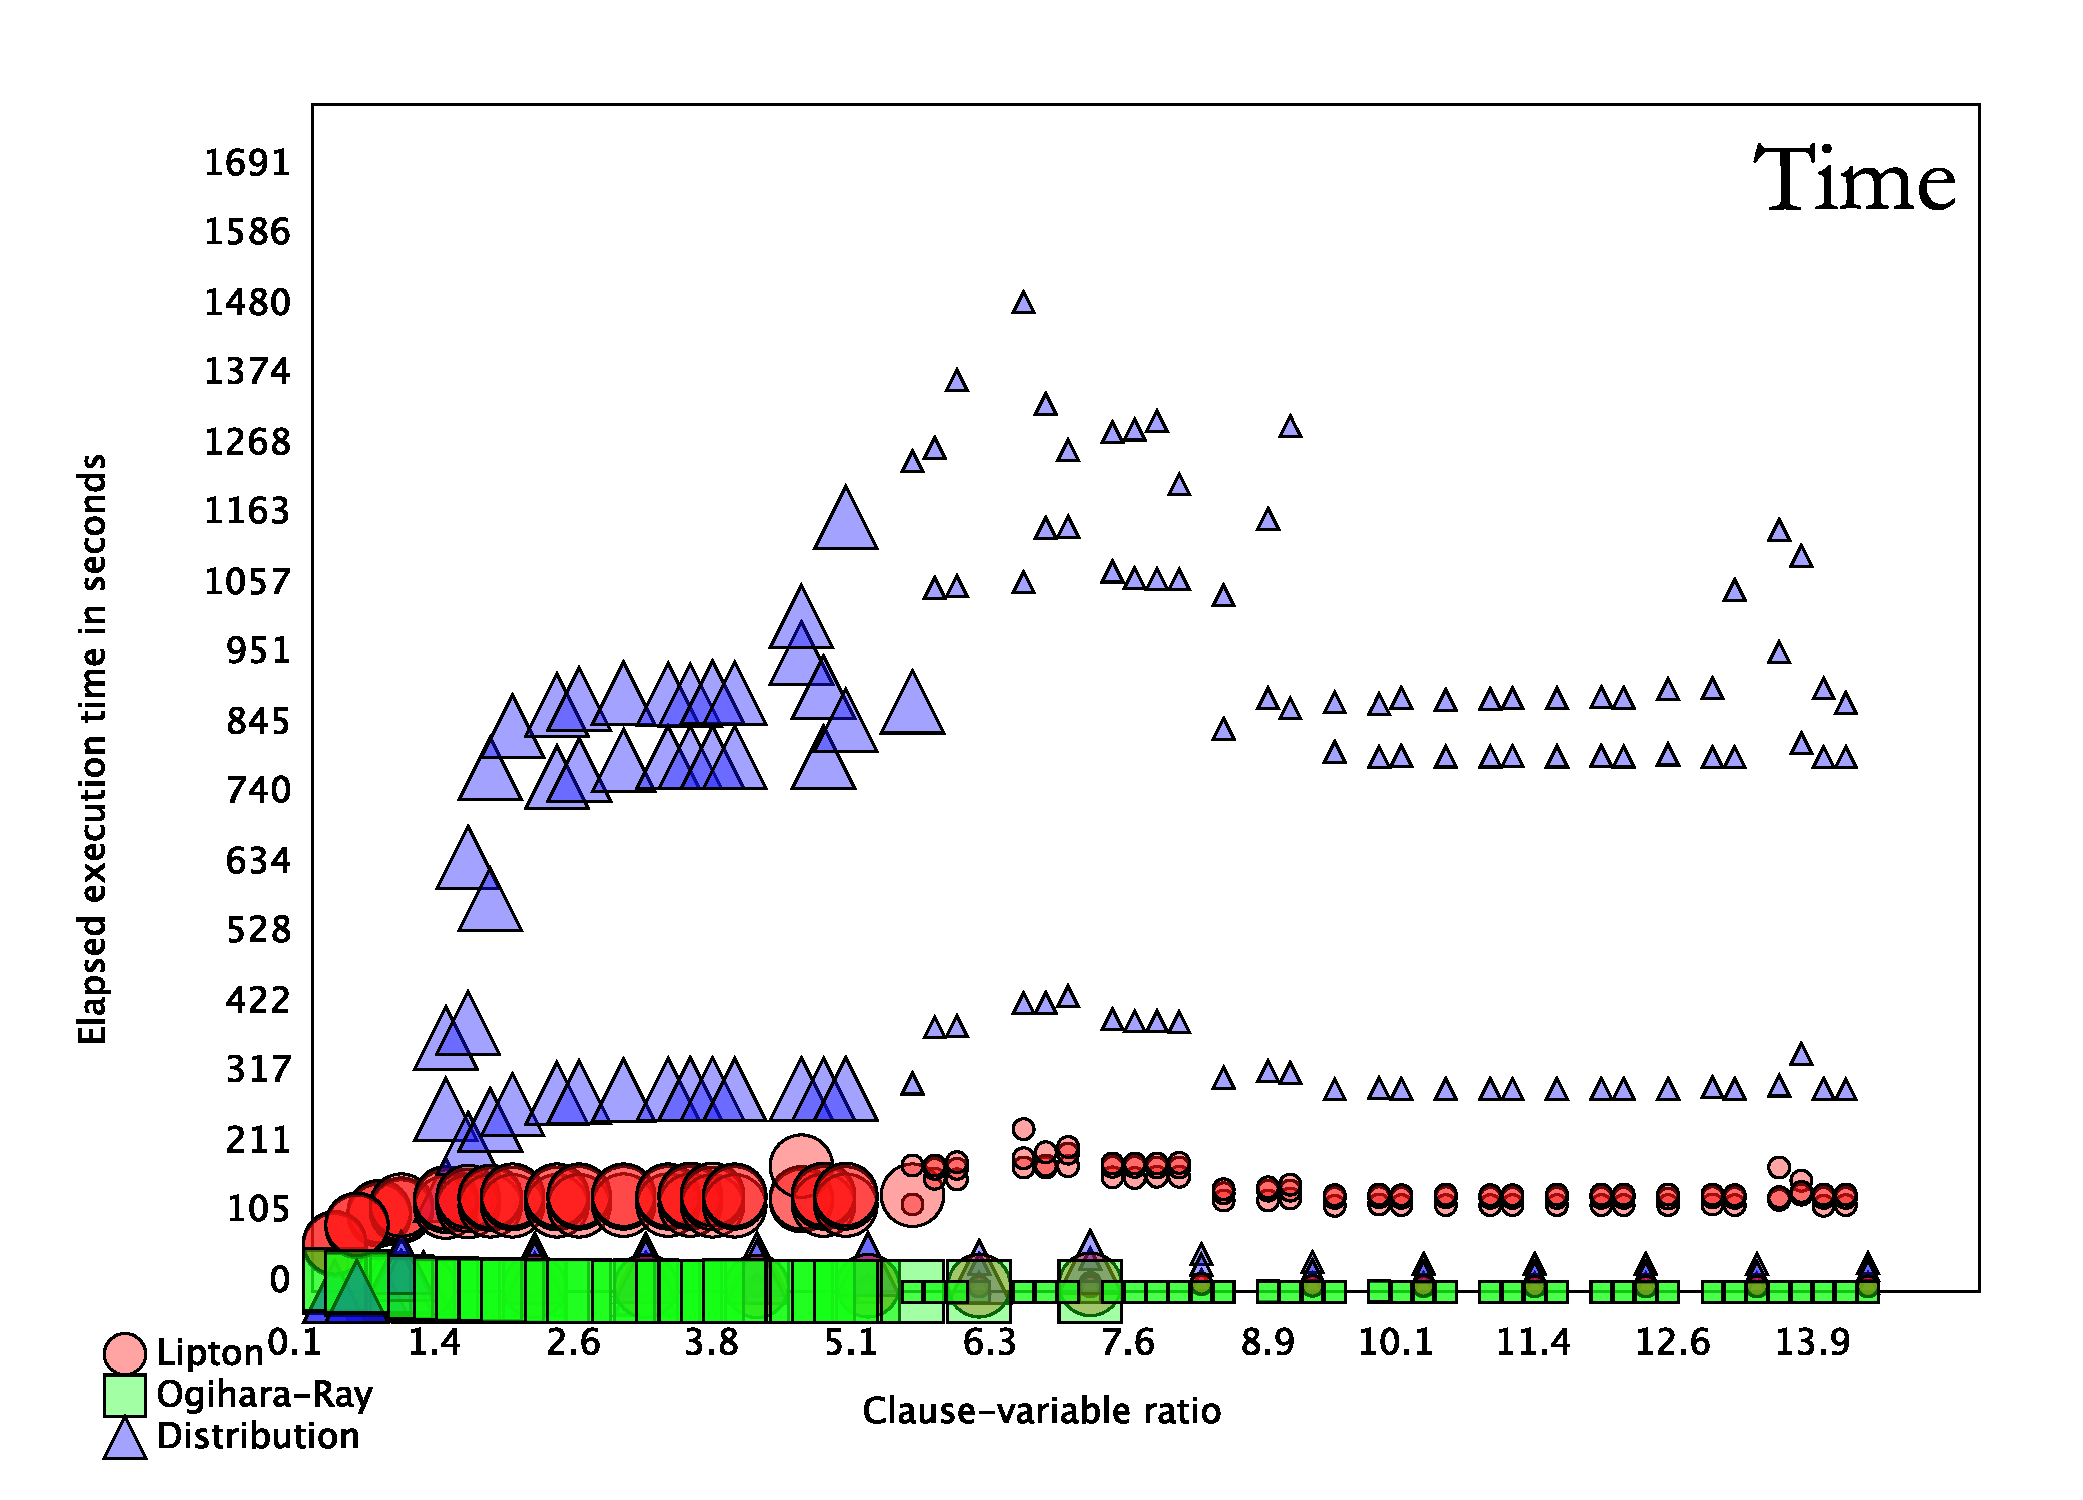
\includegraphics[width=1.1\textwidth]{./figures/metricOutput/Time.pdf}

\caption{Clause to variable ratio $\alpha$ vs. execution time in seconds }
\label{timeFig}
\end{center}
\end{figure}
%%%%%%%%%%%%%%%%%%%%%%%%%%%%%%%%%

\FloatBarrier
			
%\subsection{Solution space}
%%%%%%%%%%%%%%%%%%%%%%%%%%%%%%%%%
\begin{figure}[htdp]

\reversemarginpar{
\textbf{Memory} is a measurement of the satisfiable instance footprint returned by each algorithm measured in Bytes.\\

Lipton's and Ogihara-Ray's algorithms share the same solution footprint.

The Distribution algorithm contains a larger solution footprint after the trivially satisfiable instances with $\alpha \approx [0.2, 0.8]$.  The space provides a set of non-conflicting assignments from $\alpha \approx [0.8, 2.9]$.  Non-conflicting assignments consist of valuations for only necessary variables. \\

Each {\sc Satisfiability} instance has a constrained solution space during the phase-transition region.  All three algorithms share the same footprint.  There are no satisfiable instances in this test with $\alpha > 7.2$. The axis in Figure \ref{memoryFig} scales accordingly.
}


\begin{center}

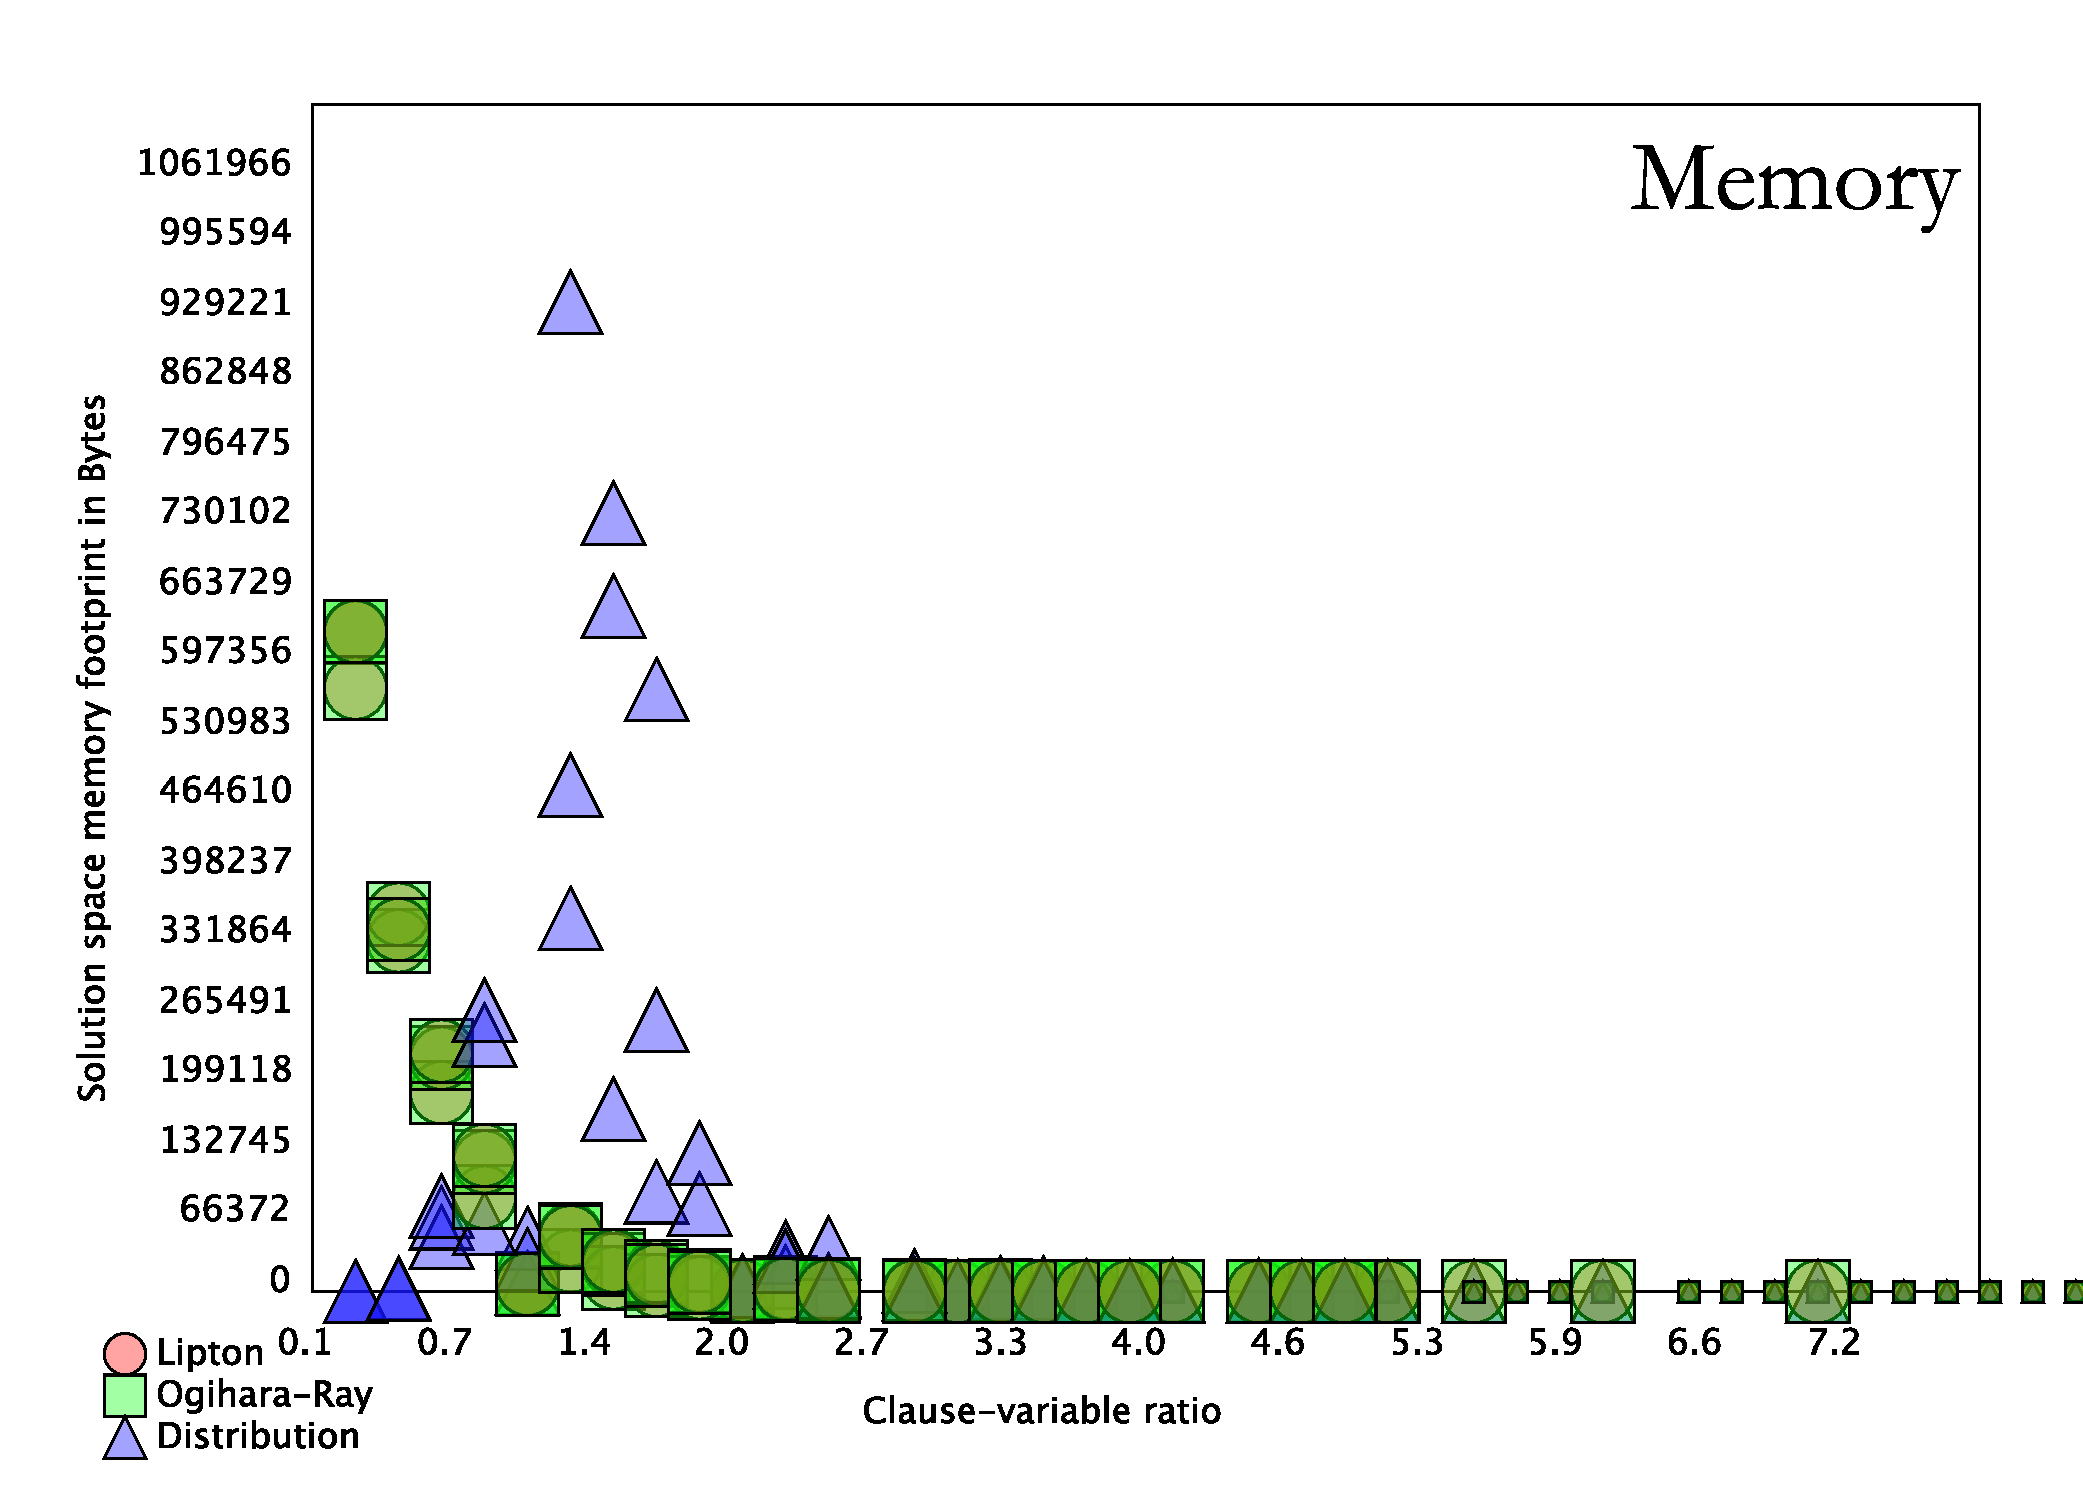
\includegraphics[width=1.1\textwidth]{./figures/metricOutput/Memory.pdf}

\caption{Clause to variable ratio $\alpha$ vs. satisfiable solution footprint in Bytes }
\label{memoryFig}
\end{center}
\end{figure}
%%%%%%%%%%%%%%%%%%%%%%%%%%%%%%%%%

\FloatBarrier

